



\section{Băm dữ liệu bằng tay thuật toán SHA-256}
M = \textbf{ANHKHOI} \\

Quy trình băm của SHA-256 được mô tả qua hai công đoạn chính:
\begin{itemize}
	\item \textbf{Tiền xử lý (Preprocessing)}: Thực hiện đệm thông điệp (padding messages), phân tách dữ liệu đã được đệm thành các khối có kích thước cố định và thiết lập các giá trị khởi tạo ban đầu nhằm phục vụ cho tính toán băm.
	\item \textbf{Tính toán băm (Hash computation}): Tạo lịch trình tin nhắn (message schedule), kết hợp cùng các hàm logic, hằng số và phép toán trên từ mã để sinh ra các giá trị băm qua từng vòng lặp. Giá trị băm cuối cùng thu được cũng chính là đầu ra của hàm băm SHA-256.
\end{itemize}

\subsection{Các phép toán sử dụng}

Các phép Toán học được áp dụng trong các hàm logic:
\begin{table}[H]
	\centering
	\caption{Các phép toán trong SHA-256}
	\label{tab:sha256-ops}
	\begin{tabular}{|l|l|l|}
		\hline
		\textbf{Ký hiệu} & \textbf{Phép toán} & \textbf{Mô tả chi tiết} \\ \hline
		$ROTR^n(x)$ & Xoay phải & Dịch chuyển vòng tròn $x$ sang phải $n$ bit. \\ \hline
		$SHR^n(x)$ & Dịch phải & Dịch $x$ sang phải $n$ bit, lấp đầy bên trái bằng bit 0. \\ \hline
		$x \oplus y$ & XOR & Phép toán Exclusive-OR theo từng bit. \\ \hline
		$x \wedge y$ & AND & Phép toán logic AND theo từng bit. \\ \hline
		$\neg x$ & NOT & Phép lấy bù (đảo bit) của $x$. \\ \hline
		$x = (a+b) \mod 2^{32} $ & Cộng Modulo & Phép cộng số nguyên không dấu modulo $2^{32}$. \\ \hline
	\end{tabular}
\end{table}	

SHA-256 sử dụng sáu hàm logic, các hàm đều xử lý với các từ 32~bit, được biểu diễn qua $x, y$ và $z$. Đầu ra của mỗi hàm sẽ là một từ 32~bit mới.

\begin{align}
	Ch(x,y,z) &= (x\land y)\oplus(\neg x\land z) \\
	Maj(x,y,z)&= (x\land y)\oplus(x\land z)\oplus(y\land z)\\
	\Sigma_0^{\{256\}} &= ROTR^{28}(x) \oplus ROTR^{13}(x) \oplus ROTR^{22}(x)\\
	\Sigma_1^{\{256\}} &= ROTR^{6}(x) \oplus ROTR^{11}(x) \oplus ROTR^{25}(x)\\
	\sigma_0^{\{256\}} &= ROTR^{7}(x) \oplus ROTR^{18}(x) \oplus SHR^{3}(x)\\
	\sigma_1^{\{256\}} &= ROTR^{17}(x) \oplus ROTR^{19}(x) \oplus SHR^{10}(x)
\end{align}

\subsection{Tiền xử lý}

\subsubsection{Đệm tin nhắn}

Một tin nhắn $M$ (Đầu vào của thuật toán) cần phải được đệm trước khi qua công đoạn tính toán băm. Đệm tin nhắn giúp đảm bảo độ dài tin nhắn sau khi được đệm sẽ là một bội số của 512. 

Trước tiên, ta sẽ chuyển đổi đầu vào $M$ biểu diễn dưới dạng nhị phân, theo mã ASCII:

\begin{align*}
	M &= ANHKHOI \\
	\xrightarrow[Bytes]{} &= 01000001~ 01001110~ 01001000~ 01001011~ 01001000~ 01001111~ 01001001	
\end{align*}

Độ dài của tin nhắn $M ~\text{là}~ \ell = 56~ bit$, ta thêm bit 1 vào cuối tin nhắn, sau đó là $448-(56+1) = 391$ bit 0, và cuối cùng là 64~bit biểu diễn độ dài của tin nhắn dưới dạng nhị phân (56~bit).

\[
\footnotesize
\underbrace{01000001}_{\text{\textbf{"A"}}} \quad
\underbrace{01001110}_{\text{\textbf{"N"}}} \quad
\underbrace{01001000}_{\text{\textbf{"H"}}} \quad
\underbrace{01001011}_{\text{\textbf{"K"}}} \quad
\underbrace{01001000}_{\text{\textbf{"H"}}} \quad
\underbrace{01001111}_{\text{\textbf{"O"}}} \quad
\underbrace{01001001}_{\text{\textbf{"I"}}} \quad
1 \quad
\overbrace{00...00}^{391} \quad
\overbrace{00...00111000}^{64}_{\ell=56}
\]

\subsubsection{Đệm tin nhắn}

Sau khi tin nhắn đã được đệm, tin nhắn đệm này cần phải được phân tách ra thành $N$ khối $m~bit$ trước khi thực hiện tính toán hàm băm.

Với thuật toán SHA-256, tin nhắn được đệm sẽ được phân tách ra thành $N$ khối $512~bit$ ($M^{(1)}, M^{(2)},...,M^{(N)}$). Với mỗi khối đầu vào 512~bit, chúng sẽ được biểu diễn qua 16 từ 32~bit, 32~bit đầu tiên của khối tin nhắn $i$ được kí hiệu là $M_0^i$, 32~bit tiếp theo được kí hiệu là $M_1^i$, và cứ tiếp tục cho đến  $M_{15}^i$.

Vì độ dài của đầu vào tin nhắn $M$ là 56 bit nên ta chỉ thực hiện trên một khối $M^{(1)}$.

\begin{table}[h]
	\centering
	\renewcommand{\arraystretch}{1.5}
	\begin{tabular}{|l|p{6cm}|l|}
		\hline
		\textbf{Từ} & \textbf{Giá trị (Dạng Nhị phân / Hex)} & \textbf{Ghi chú} \\ \hline
		$M_0^{(1)}$ & \texttt{01000001 01001110 01001000 01001011} (\texttt{414E484B}) & Chứa 4 ký tự "ANHK" \\ \hline
		$M_1^{(1)}$ & \texttt{01001000 01001111 01001001 10000000} (\texttt{484F4980}) & Chứa "HOI" + bit \textbf{1} + bảy bit \textbf{0} \\ \hline
		$M_2^{(1)}$ & \texttt{00000000 ... 00000000} (\texttt{00000000}) & Toàn bộ là bit 0 \\ \hline
		... & ... & ... \\ \hline
		$M_{13}^{(1)}$ & \texttt{00000000 ... 00000000} (\texttt{00000000}) & Toàn bộ là bit 0 \\ \hline
		$M_{14}^{(1)}$ & \texttt{00000000 ... 00000000} (\texttt{00000000}) & 32 bit cao của độ dài tin nhắn gốc \\ \hline
		$M_{15}^{(1)}$ & \texttt{00000000 00000000 00000000 00111000} (\texttt{00000038}) & 32 bit thấp của độ dài tin nhắn gốc (56) \\ \hline
	\end{tabular}
	\caption{Phân tách Khối $M^{(1)}$ (512 bit) sau khi đệm tin nhắn}
\end{table}

\subsection{Khởi tạo giá trị băm}
Trước khi tính toán băm, cần phải thiết lập giá trị băm khởi tạo $H^{(0)}$.

Giá trị băm khởi tạo $H^{(0)}$ trong thuật toán SHA-256, bao gồm 8 từ 32~bit được biểu diễn dưới dạng thập lục phân.

Tám từ này tương ứng với 32~bit đầu tiên của phần thập phân của căn bậc hai tám số nguyên tố đầu tiên. 

\begin{align*}
	H_0^{(0)} &= \sqrt{2} = 6a09e667 \\
	H_1^{(0)} &= \sqrt{3} = bb67ae85 \\
	H_2^{(0)} &= \sqrt{5} = 3c6ef372 \\
	H_3^{(0)} &= \sqrt{7} = a54ff53a \\
	H_4^{(0)} &= \sqrt{11} = 510e527f \\
	H_5^{(0)} &= \sqrt{13} = 9b05688c \\
	H_6^{(0)} &= \sqrt{17} = 1f83d9ab \\
	H_7^{(0)} &= \sqrt{19} = 5be0cd19 \\	
\end{align*}

\subsection{Mở rộng lịch trình tin nhắn}

Sau quá trình tiền xử lý, với mỗi khối tin nhắn $M^{(1)}, M^{(2)},...,M^{(N)}$, sẽ được xử lý theo tuần tự qua các bước sau:

\begin{enumerate}[label=\textbf{Bước \arabic*:}, leftmargin = 2.5cm]
	\item Mở rộng lịch trình tin nhắn $\{W_t\}$:
	\[
	W_t = \begin{cases} 
		M_t^{(i)} & 0 \leq t \leq 15 \\
		\sigma_1^{\{256\}}(W_{t-2}) + W_{t-7} + \sigma_0^{\{256\}}(W_{t-15}) + W_{t-16} & 16 \leq t \leq 63 
	\end{cases}
	\]
	Với $M_t^{(i)}$ là từ được lấy từ khối tin nhắn 512~bit và $W_t$ là từ 32~bit được tạo từ công thức trên.

16 từ $W_t$ đầu tiên được lấy ra từ khối tin nhắn 512~bit $M^(1)$, các từ còn lại được tạo ra thông qua việc tính toán dựa trên công thức.

\textbf{Ví dụ:} Tính từ thứ 17 $W_{16}$:
\begin{center}
	$W_{16} = \sigma_1^{\{256\}}(W_{14}) + W_{9} + \sigma_0^{\{256\}}(W_{1}) + W_{0}$
\end{center}
{Với:
\begin{align*}
	W_{14} &= \text{0x00000000} \implies \sigma_1^{\{256\}}(W_{14}) = \text{0x00000000} \\
	W_{1} &= \text{0x484F4980} \\
	&\implies \sigma_0^{\{256\}}(W_{1}) = ROTR^{7}(W_1) \oplus ROTR^{18}(W_1) \oplus SHR^{3}(W_1) \\
	&\implies \sigma_0^{\{256\}}(W_{1}) = \text{0x00909E93} \oplus \text{0xD2601213} \oplus \text{0x0909E930}\\
	&\implies \sigma_0^{\{256\}}(W_{1}) = \text{0xDBF965B0}
\end{align*}
Vậy: 
{	\small
	\begin{align*}
	W_{16} &= \text{0x00000000} + \text{0x00000000} + \text{0xDBF965B0} + \text{0x414E484B}\pmod {\text{0x100000000}}\\ 
	 W_{16} &= \text{0x11D47ADFB} {\pmod {\text{0x100000000}}} = \text{0x1D47ADFB}   
\end{align*}}
Thực hiện tương tự với các từ khóa từ $W_{17},...,W_{63}$

\item Khởi tạo biến làm việc $a,b,c,d,e,f,g,h$, tại vòng nén đầu tiên các biến làm việc này cũng tương ứng với 32 bit phần thập phân của căn bậc hai 8 số nguyên tố đầu tiên.

\begin{align*}
	a &= H_0^{(0)} = \sqrt{2} = 6a09e667 \\
	b &= H_1^{(0)} = \sqrt{3} = bb67ae85 \\
	c &= H_2^{(0)} = \sqrt{5} = 3c6ef372 \\
	d &= H_3^{(0)} = \sqrt{7} = a54ff53a \\
	e &= H_4^{(0)} = \sqrt{11} = 510e527f \\
	f &= H_5^{(0)} = \sqrt{13} = 9b05688c \\
	g &= H_6^{(0)} = \sqrt{17} = 1f83d9ab \\
	h &= H_7^{(0)} = \sqrt{19} = 0x5be0cd19 \\	
\end{align*}

Một vòng nén sẽ diễn ra như sau:
\begin{itemize}
	\item 	\begin{align*}
		T_1 &= h + \Sigma_1^{\{256\}}(e)+Ch(e,f,g)+K_t^{\{256\}}+ W_t \\
		T_2 &= \Sigma_0^{\{256\}}(a) + Maj(a,b,c) \\
		h &= g \\
		g &= f \\
		f &= e \\
		e &= d + T_1 \\
		d &= c\\
		c &= b\\
		b &= a\\
		a &= T_1 + T_2
	\end{align*}
	Trong đó:
	\begin{itemize}
		\item $T_1~ \text{và} ~T_2$: Hai biến tạm được sử dụng để tính toán theo từng chu kỳ.
		\item $a,b,c,d,e,f,g,h$: Các biến làm việc.
		\item $K_t^{\{256\}}$: Hằng số theo chu kỳ $t$.
		\item $W_t$: Từ trong lịch trình tin nhắn.
	\end{itemize}
	\item Tính toán giá trị băm trung gian $H^{(i)}$ thứ $i$:
	\begin{align*}
		H_0^{(i)} &= a + H_0^{(i-1)} \quad & H_4^{(i)} &= e + H_4^{(i-1)} \\
		H_1^{(i)} &= b + H_1^{(i-1)} \quad & H_5^{i} &= f + H_5^{(i-1)} \\
		H_2^{(i)} &= c + H_2^{(i-1)} \quad & H_6^{(i)} &= g + H_6^{(i-1)} \\
		H_3^{(i)} &= d + H_3^{(i-1)} \quad & H_7^{(i)} &= h + H_7^{(i-1)}
	\end{align*}
\end{itemize}

\textbf{Ví dụ}: Thực hiện vòng nén thứ nhất:
\begin{align*}
T_1 &= h + \Sigma_1^{\{256\}}(e)+Ch(e,f,g)+K_t^{\{256\}}+ W_t\\ 
T_2 &= \Sigma_0^{\{256\}}(a) + Maj(a,b,c) \\
\end{align*}
Trong đó:
\begin{align*}
	Ch(e,f,g) &= (e\land f) \oplus (\neg e\land g)\\
	&= (\text{0x510e527f} \land \text{0x9b05688c}) \oplus (\neg \text{0x510e527f} \land \text{0x1f83d9ab}) \\
	&= \text{0x1104400c} \oplus (\text{0xaef1ad80} \land \text{0x1f83d9ab}) \\
	&= \text{0x1104400c} \oplus \text{0x0e818980} = \text{0x1f85c98c} 
\end{align*}
\begin{align*}
\Sigma_1^{{256}}(e) &= ROTR^6(e) \oplus ROTR^{11}(e) \oplus ROTR^{25}(e) \\
	&= \text{0xfd443949} \oplus \text{0x4fea21ca} \oplus \text{0x87293fa8} \\
	&= \text{0x3587272b}
\end{align*}
\begin{align*}
\Sigma_0^{{256}}(a) &= ROTR^2(a) \oplus ROTR^{13}(a) \oplus ROTR^{22}(a) \\
	&= \text{0xda827999} \oplus \text{0x333b504f} \oplus \text{0x27999da8} \\
	&= \text{0xce20b47e}
\end{align*}
\begin{align*}
	Maj(a,b,c) &= (a \land b) \oplus (a \land c) \oplus (b \land c) \\
	&= \text{0x2a01a605} \oplus \text{0x2808e262} \oplus \text{0x3866a200} \\
	&= \text{0x3a6fe667}
\end{align*}

	\begin{align*}
		T_1 &= (h + \Sigma_1^{\{256\}}(e) + Ch(e, f, g) + K_0^{\{256\}} + W_0) \pmod{\text{0x100000000}} \\
		&= (\text{0x5be0cd19} + \text{0x3587272b} + \text{0x1f85c98c} \\
		&\quad + \text{0x428a2f98} + \text{0x414e484b}) \pmod{\text{0x100000000}} \\
		&= \text{0x134c635b3} \pmod{\text{0x100000000}} \\
		&= \text{0x34c635b3}
	\end{align*}

Ta tính được $T_1$ và $T_2$:
\begin{align*}
	T_2 &= (\Sigma_0^{{256}}(a) + Maj(a, b, c)) \pmod{\text{0x100000000}} \\
	&= (\text{0xce20b47e} + \text{0x3a6fe667}) \pmod{\text{0x100000000}} \\
	&= \text{0x108909ae5} \pmod{\text{0x100000000}} \\
	&= \text{0x08909ae5}
\end{align*}

Tiến hành cập nhật các biến làm việc theo thứ tự sau:
\begin{align*}
	h &= g = \text{0x1f83d9ab} \\
	g &= f = \text{0x9b05688c} \\
	f &= e = \text{0x510e527f} \\
	e &= (d + T_1) \pmod{\text{0x100000000}} = \text{0xda162aed} \\
	d &= c = \text{0x3c6ef372} \\
	c &= b = \text{0xbb67ae85} \\
	b &= a = \text{0x6a09e667} \\
	a &= (T_1 + T_2) \pmod{\text{0x100000000}} = \text{0x3d56d098}
\end{align*}

Cập nhật giá trị băm trung gian, thực hiện trên phép cộng số nguyên modulo $2^{32}$:

{\small
	\begin{align*}
		H_0^{(1)} &= \text{0x6a09e667} + \text{0x3d56d098} = \text{0xa760b6ff} \\
		H_1^{(1)} &= \text{0xbb67ae85} + \text{0x6a09e667} = \text{0x257194ec} \\
		H_2^{(1)} &= \text{0x3c6ef372} + \text{0xbb67ae85} = \text{0xf7d6a1f7} \\
		H_3^{(1)} &= \text{0xa54ff53a} + \text{0x3c6ef372} = \text{0xe1beeaac} \\
		H_4^{(1)} &= \text{0x510e527f} + \text{0xda162aed} = \text{0x2b247d6c} \\
		H_5^{(1)} &= \text{0x9b05688c} + \text{0x510e527f} = \text{0xec13bb0b} \\
		H_6^{(1)} &= \text{0x1f83d9ab} + \text{0x9b05688c} = \text{0xba894237} \\
		H_7^{(1)} &= \text{0x5be0cd19} + \text{0x1f83d9ab} = \text{0x7b64a6c4}
	\end{align*}
}

\item Thực hiện quá trình nén 64 lần, sau mỗi quá trình nén ta sẽ cập nhật giá trị băm trung gian $H^{(i)}$ thứ ${i}$, đầu ra của hàm băm chính là giá trị băm trung gian sau khi thực hiện vòng nén cuối cùng.
\end{enumerate}

Tại vòng cuối cùng, giá trị hàm băm trung gian như sau:
{\small
	\begin{align*}
		H_0^{(63)} &= \text{0xf738cde4} \quad & H_4^{(63)} &= \text{0x8564cab9} \\
		H_1^{(63)} &= \text{0x246b38b5} \quad & H_5^{(63)} &= \text{0x6422e583} \\
		H_2^{(63)} &= \text{0xad46bc2d} \quad & H_6^{(63)} &= \text{0x2a1d4ab0} \\
		H_3^{(63)} &= \text{0xe7dc3e18} \quad & H_7^{(63)} &= \text{0xb632a094}
	\end{align*}
}

Các giá trị trung gian này cũng chính là đầu ra của quá trình băm tin nhắn sử dụng SHA-256. Thực hiện nối bytes các giá trị trung gian này lại, ta thu được đầu ra:

\begin{align*}
	 \text{SHA\_256\_Output} &= H_0 \parallel H_1 \parallel H_2 \parallel H_3 \parallel H_4 \parallel H_5 \parallel H_6 \parallel H_7 \\ &= f738cde4246b38b5ad46bc2de7dc3e188564cab96422e5832a1d4ab0b632a094
\end{align*}

\section{Kiểm chứng kết quả}

Để kiểm tra quá trình băm dữ liệu bằng tay có chính xác hay không, việc kiểm chứng sẽ sử dụng hai phương pháp chính để kiểm tra:
\begin{itemize}
	\item Sử dụng thư viện chuẩn \texttt{hashlib}.
	\item Sử dụng thuật toán SHA-256 được triển khai từ đầu, không dùng thư viện ngoài nào khác.
\end{itemize}

Cả hai phương pháp đều trả về cùng một kết quả băm, với cùng đầu vào plaintext như đã đề cập ở phần giải tay. 

\begin{figure}[H]
	\centering
	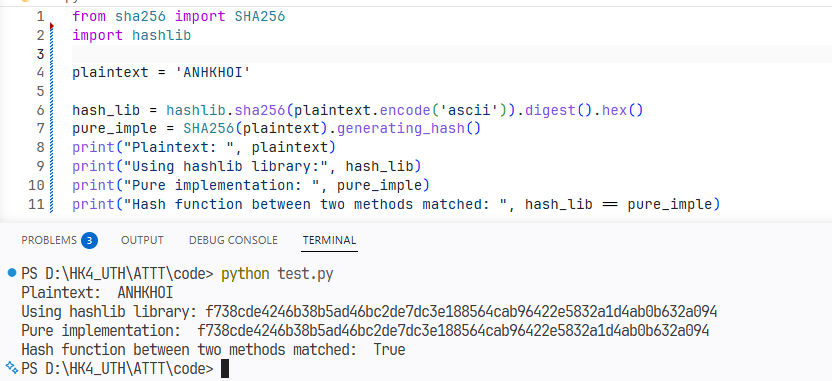
\includegraphics[width=\textwidth]{result.png}
	\caption{Kết quả kiểm chứng}
	\label{fig:result}
\end{figure}

